\chapter{Implementation}
\label{sec:implementation}

\section{Introduction}
This section has outlined the three essential modules that constitute the DroneDSL, covering the complete pipeline of the project. These modules are:
\begin{itemize}
    \item \textbf{Preprocessing}: Prepares the initial data and configurations needed for the subsequent stages.
    \item \textbf{Compilation}: Translates the DroneDSL script into an executable format, creating an Abstract Syntax Tree and subsequently generating a task automata structure.
    \item \textbf{Runtime}: Manages the execution of tasks during drone operations, overseeing the mission control and task transitions based on real-time condition.
\end{itemize}
\section{Preprocessing}
\subsection{Overview}
During this phase, the system processes a KML file to extract waypoints necessary for takeoff and flight tasks. These waypoints are bound to variable names designated by the user. In addition, users are required to compose their own DSL scripts to generate the configurations needed for their specific flight missions.
\begin{figure}[H] % The 'h' here is a placement specifier (here)
    \centering % This centers the figure
    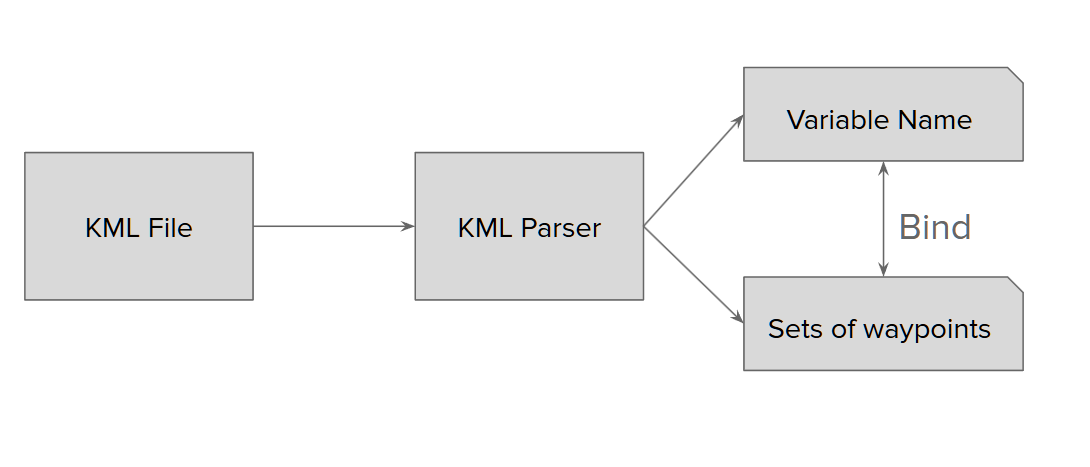
\includegraphics[width=0.8\textwidth]{Pictures/pre_flow.PNG}
    \caption{Workflow Diagram for Preprocess Module.}
    \label{fig:workflow_diagram}
\end{figure}

\subsection{Workflow}
\begin{itemize}
    \item Initially, users must generate the flight route using a mapping service or a ground control station.~\ref{fig:flight_route} is an example where Google My Maps is used to delineate a flight route for a mission.
    
    \begin{figure}[H] % The 'h' here is a placement specifier (here)
        \centering % This centers the figure
        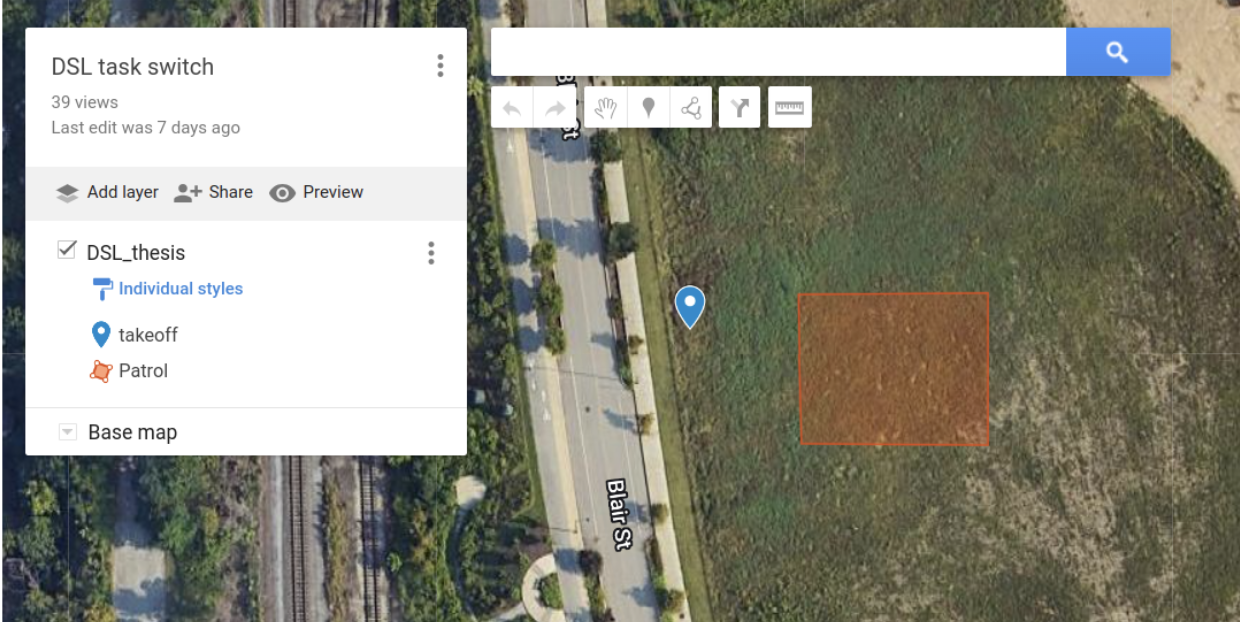
\includegraphics[width=0.8\textwidth]{Pictures/pre_qgc.PNG}
        \caption{Example of a flight route designed using Google My Maps.}
        \label{fig:flight_route}
    \end{figure}
    
    \item After the flight route is drawn, it is converted into a KML file. KML is retained in our pipeline due to its efficiency in expressing geographical information. It is used solely to represent waypoint information.~\ref{fig:kml_script} is a segment of the KML script that corresponds to the flight route illustrated in~\ref{fig:flight_route}.
    \begin{figure}[H] % The 'h' here is a placement specifier (here)
        \centering % This centers the figure
        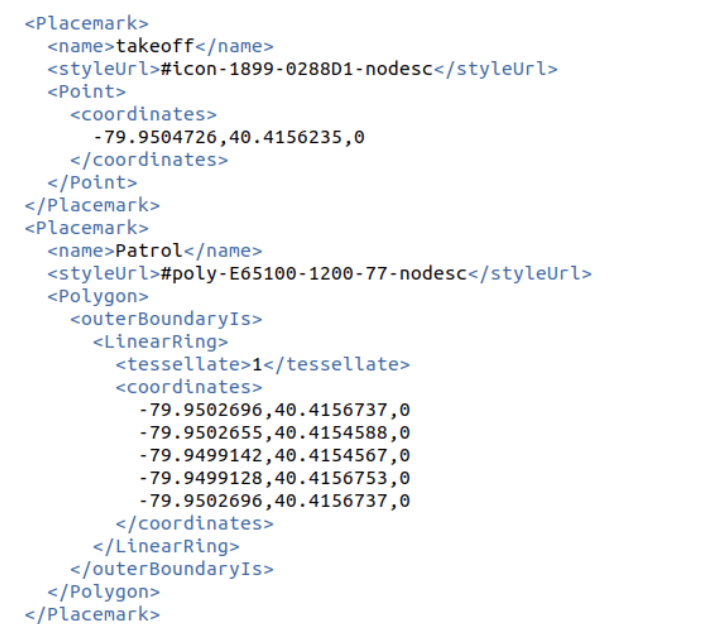
\includegraphics[width=0.8\textwidth]{Pictures/pre_kml.PNG}
        \caption{Snippet of the KML script for the depicted flight route.}
        \label{fig:kml_script}
    \end{figure}
    \item Once the KML file is obtained, the DroneDSL utilizes a KML parser to extract the waypoints and the names of the areas associated with these waypoints. These details are then bound together, allowing users to reference a set of waypoints using a single Waypoints ID. This approach significantly reduces the cognitive effort required to input each waypoint manually. ~\ref{fig:workflow_diagram} illustrates the workflow following the acquisition of the KML file.
\end{itemize}


\section{Compilation}
\subsection{Overview}
The DroneDSL script is interpreted into an Abstract Syntax Tree (AST). This AST is subsequently transformed into a Task Automata data structure in memory, which is then converted into a format suitable for integration with drone software development kits (SDKs).~\ref{fig:cli_flow} depicts the entire workflow of the compilation process.
\begin{figure}[H] % The 'h' here is a placement specifier (here)
    \centering % This centers the figure
    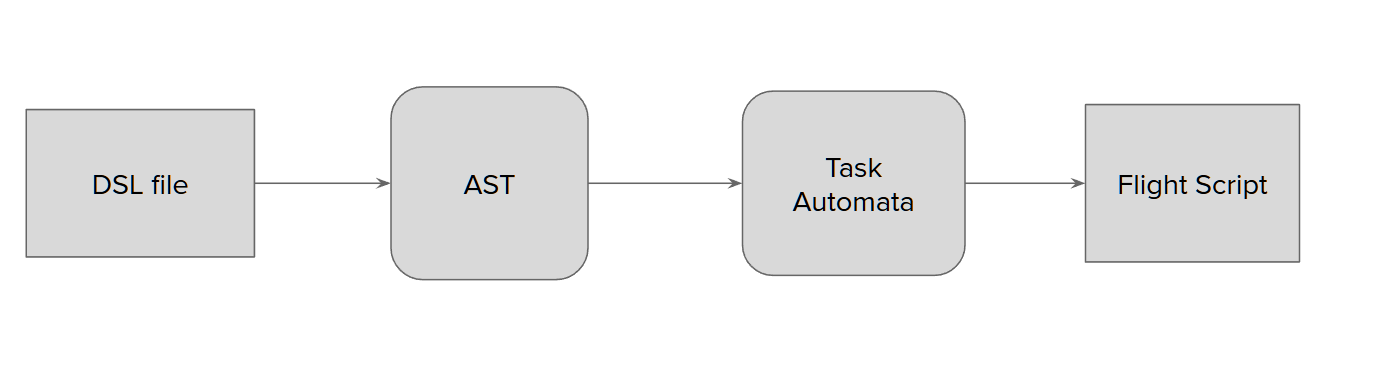
\includegraphics[width=0.8\textwidth]{Pictures/cli_flow.PNG}
    \caption{Workflow Diagram for Compilation Module.}
    \label{fig:cli_flow}
\end{figure}
\subsection{Compiler Details}
\subsubsection{Lexical Analysis}
The lexical analyzer processes the DroneDSL input and generates tokens based on the following specifications:
\begin{itemize}
    \item \textbf{Number}: Identifies integers and floating-point numbers. It matches an optional negative sign followed by one or more digits, possibly including a decimal point followed by more digits.
    \item \textbf{Identifier}: Recognizes identifiers comprising Greek (\textgreek{α}-\textgreek{ω}) and Latin (a-zA-Z) letters, underscores, digits, apostrophes, and hyphens, starting with a letter or underscore.
    \item \textbf{EOL}: Represents end-of-line characters.
    \item \textbf{White Space}: Defines whitespace characters, including spaces and tabs.
    \item \textbf{Keywords and Symbols}: Captures DSL keywords such as "Task," "Detect," "Track," "Mission," "Transition," "Start" and symbols like \texttt{\{ \} ( ) [ ] , : -> < >}.
    \item \textbf{Bad Character}: This rule captures any character input that does not match any of the specified patterns.
\end{itemize}

\begin{lstlisting}[style=c1]
    EOL=\R
    WHITE_SPACE=\s+
    NUMBER=-?[0-9]+(\.[0-9]+)?
    IDENTIFIER=
        [(alpha)-(omega)a-zA-Z_][(alpha)-(omega)a-zA-Z0-9_'-]*
    
    %%
    <YYINITIAL> {
      {WHITE_SPACE}       { return WHITE_SPACE; }
      {NUMBER}            { return NUMBER; }
      Task                { return TASK_KW; }
      Detect              { return TASK_DETECT_KW; }
      Track               { return TASK_TRACK_KW; }
      Avoid               { return TASK_AVOID_KW; }
      Mission             { return MISSION_KW; }
      Transition          { return TRANSITION_KW; }
      Start               { return MISSION_START_KW; }
      {IDENTIFIER}        { return ID; }
      "{"                 { return LBRACE; }
      "}"                 { return RBRACE; }
      "("                 { return LPAREN; }
      ")"                 { return RPAREN; }
      "["                 { return LSQUA; }
      "]"                 { return RSQUA; }
      ","                 { return COMMA; }
      ":"                 { return COLON; }
      "->"                { return ARROW; }
      "<"                 { return LANGL; }
      ">"                 { return RANGL; }
    }
    
    [^] { return BAD_CHARACTER; }
\end{lstlisting}

\subsubsection{Parsing}
DroneDSL uses context free grammar to define constructs for files, tasks, and missions, with components like task name, attribute, and mission transition. Each major component is structured as follows:
\begin{itemize}
    \item File Structure
    \begin{itemize}
        \item File: A file consists of a task followed by a mission.
    \end{itemize}
    \begin{lstlisting}[style=customgo]
    // file structure
    file ::= task mission
    \end{lstlisting}
    
    \item Task Definition
    \begin{itemize}
        \item \textbf{Task}: Defined by a keyword (TASK\_KW) followed by a series of task declarations (task\_decl) enclosed in braces.
        \item \textbf{Task Declaration}: A declaration can be for detecting, tracking, or avoiding (TASK\_DETECT\_KW, TASK\_TRACK\_KW, TASK\_AVOID\_KW), followed by a Task Name and a Task Body.
        \item \textbf{Task Body}: Consists of attributes separated by commas and enclosed in braces.
        \item \textbf{Attribute}: A sequence of attributes where each attribute is identified by an ID followed by a colon and an attribute expression.
        \item \textbf{Attribute Expression}: The expression for an attribute, which could be a number, a name, a list of waypoints, a waypoints variable, etc.
        \item \textbf{Task Name and Name}: Both are defined as IDs.
    \end{itemize}
    \begin{lstlisting}[style=customgo]
    // defining the task
    task ::= TASK_KW <<braced task_decl*>>
    task_decl ::= (TASK_DETECT_KW | TASK_TRACK_KW) task_name task_body
    task_body ::= <<braced <<commaSep attributes>>>>
    private attributes ::= attribute*
    attribute ::=  ID <<coloned attribute_expr>>
    attribute_expr ::= NUMBER | name | <<square_bracked <<commaSep <<paren tuple>> >> >> | <<angle_bracked name>> | <<paren tuple>>
    tuple ::= NUMBER COMMA NUMBER COMMA NUMBER
    task_name ::= name
    name ::= ID
    \end{lstlisting}    
    \item Mission Definition
    \begin{itemize}
        \item \textbf{Mission}: Defined by a keyword (MISSION\_KW) followed by content enclosed in braces.
        \item \textbf{Mission Content}: Consists of a mission\_start\_decl followed by zero or more mission\_transitions.
        \item \textbf{Start Transition}: Starts with a keyword (MISSION\_START\_KW) followed by a task\_name.
        \item \textbf{Task Transition}: Defined by a TRANSITION\_KW, a condition in parentheses, a task\_name, an arrow (ARROW), and another task\_name.
        \item \textbf{Transition Argument}: A condition which is an ID possibly followed by a number or another ID in parentheses.
    \end{itemize}
    \begin{lstlisting}[style=customgo]
    // defining the mission
    mission ::= MISSION_KW <<braced mission_content>>
    mission_content ::= mission_start_decl mission_transition*
    mission_start_decl ::= MISSION_START_KW task_name
    mission_transition ::= TRANSITION_KW <<paren cond>> task_name ARROW task_name
    cond ::= ID <<paren (NUMBER | ID) >>?
    \end{lstlisting}
    \item Meta Rules \\
    These rules define how lists and groups are structured:
    \begin{itemize}
        \item \textbf{Parentheses}: Content enclosed in parentheses.
        \item \textbf{Angle Brackets}: Content enclosed in angle brackets.
        \item \textbf{Square Brackets}: Content enclosed in square brackets.
        \item \textbf{Colon}: A colon followed by some content.
        \item \textbf{Comma Separation}: A comma-separated list of items.
        \item \textbf{Braces}: Content enclosed in braces.
    \end{itemize}
    \begin{lstlisting}[style=customgo]
    // meta rules
    meta paren ::= LPAREN <<param>> RPAREN
    meta angle_bracked ::= LANGL <<param>> RANGL
    meta square_bracked ::= LSQUA <<param>> RSQUA
    private meta coloned ::= COLON <<param>>
    private meta commaSep ::= <<param>> (COMMA <<param>>) *
    private meta braced ::= LBRACE <<param>> RBRACE
    \end{lstlisting}
\end{itemize}


\subsection{Semantic Analysis}
Once the DroneDSL script is parsed, the Abstract Syntax Tree (AST) is transformed into a Flight Plan Structure (FPS), which effectively represents the task automata within the system memory. This structure encompasses a starting task identifier and an array of Task objects, each carefully defined by the users with the necessary attributes for successful task execution.~\ref{fig:cli_auto} visually depicts the FPS. The FPS is then utilized by DroneDSL to synthesize mission code that is compatible with the drone SDK.

\begin{figure}[H] % The 'h' here is a placement specifier (here)
    \centering % This centers the figure
    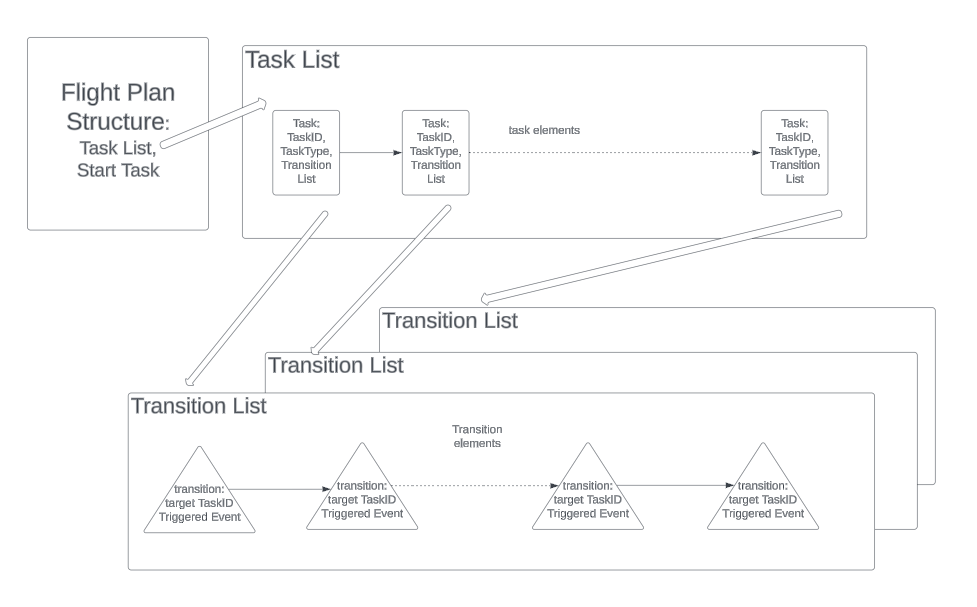
\includegraphics[width=0.8\textwidth]{Pictures/cli_auto.PNG}
    \caption{Flight Plan Structure (FPS).}
    \label{fig:cli_auto}
\end{figure}

\begin{itemize}
    \item \textbf{Flight Plan Structure (FPS)}: Comprises the start task ID and a comprehensive list of tasks. This structure serves as the backbone for task management and transition flow within the mission.
    \item \textbf{Task List}: This component includes each task object created and defined by the user, forming the operational sequence for the mission.
    \item \textbf{Task}: Every task object within the list includes a unique task ID, task type (such as detect, track, or avoid), and a list of transitions that define the flow to subsequent tasks based on specific events.
    \item \textbf{Transition List}: Contains all transitions associated with a task object, detailing the conditions under which a transition to another task is triggered.
    \item \textbf{Transition}: Each transition specifies the event that triggers it and the ID of the next task to be executed.
\end{itemize}


\section{Runtime}
\subsection{Overview}
DroneDSL requires an entry-point file created using the drone SDK to establish drone connectivity and initiate external communications. This activates the mission controller, a DroneDSL library module that oversees the entire mission. It manages the task runner, an asynchronous worker responsible for starting and stopping tasks. Tasks are performed asynchronously, executing drone commands and monitoring events through transition threads. Triggered events are reported to the mission controller, which assesses them and instructs the task runner to either switch, continue, or terminate tasks. Upon command, the task runner stops all current tasks and transitions.

\begin{figure}[H] % The 'h' here is a placement specifier (here)
    \centering % This centers the figure
    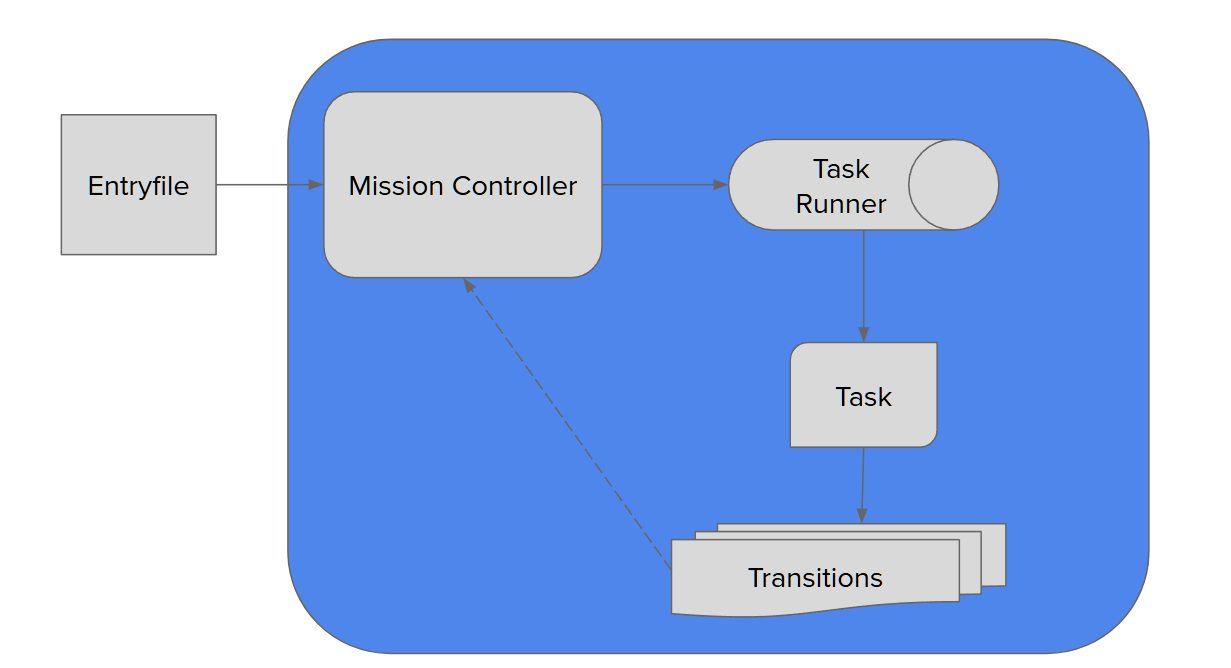
\includegraphics[width=0.8\textwidth]{Pictures/run_flow.PNG}
    \caption{Workflow Diagram for the Runtime Module.}
    \label{fig:runtime_diagram}
\end{figure}

\subsection{Components}
\begin{itemize}
    \item \textbf{Mission Controller}: Oversees the entire flight operation.
    \begin{itemize}
        \item Initiates the mission by launching the task runner and instructing the drone to take off.
        \item Modifies tasks in response to events detected during task transitions, guided by the mission creator.
        \item Concludes the mission by shutting down the task runner and directing the drone to return.
    \end{itemize}
    \item \textbf{Task Runner}: Operated by the mission controller to execute or end tasks.
    \begin{itemize}
        \item Manages a queue of tasks, executing new tasks as they are introduced.
        \item Capable of ending the current task and initiating subsequent ones.
    \end{itemize}
    \item \textbf{Mission Creator}: An automatically generated file that details the specific mission set-up by DroneDSL.
    \begin{itemize}
        \item Defines the task automata, providing a reference for the mission controller.
    \end{itemize}
\end{itemize}

